\section{OpenGeoSys - Finite-Element-Method}
\label{app:ogs}

\begin{wrapfigure}{l}{6cm}
  \centering
  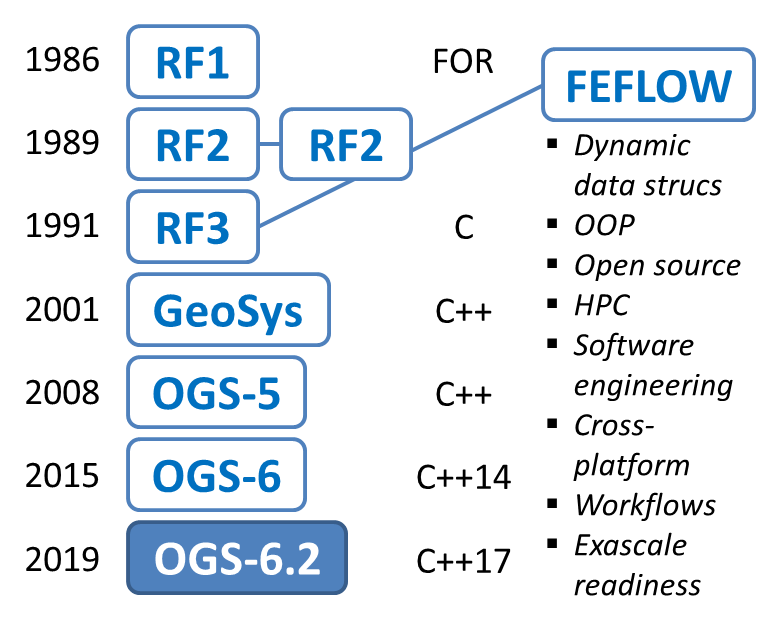
\includegraphics[width=6cm]{figures/ogs-2019}
  \caption{OpenGeoSys development history}
  \label{fig:ogs-history}
\end{wrapfigure}
OpenGeoSys (OGS) is a scientific open-source initiative for the numerical simulation of thermo-hydro-mechanical/chemical (THMC) processes in porous and fractured media, inspired by FEFLOW \cite{Diersch2014} and ROCKFLOW concepts and continuously developed since the mid-eighties (Fig. \ref{fig:ogs-history}), see e.g. \cite{Kolditz:1990}, \cite{Wollrath:1990}, \cite{Kroehn:1991} and \cite{Helmig:1993}. Meanwhile, more than 50 PhD projects have been dedicated to the OGS development since the merger in the nineties.

The OGS framework is targeting applications of various disciplines in environmental geoscience, e.g., in the fields of regional \cite{Jing20181989}, contaminant \cite{Nixdorf2017598} and coastal hydrology \cite{Walther2017648}, fundamental geothermal processes \cite{Parisio2019} and geothermal energy systems \cite{Meng2018971,HEIN201680}.
%
OGS is applied for energy storage applications in technical systems such as concrete \cite{Miao2019977} or  zeolite-based heat storage \cite{Lehmann20191102} and natural systems such as salt caverns \cite{Bottcher2017,Nagel2017}. 
%
OGS is also used in fundamental studies for nuclear waste management \cite{Shao201933}.

The most recent version, OpenGeoSys-6 (OGS-6) \cite{Naumov:2018,Bilke2019}, is a complete re-implementation of the multi-physics code OpenGeoSys-4/5 \cite{Kolditz2004225,Wang:2006} using advanced methods in software engineering and architecture with a focus on code quality, modularity, performance and comprehensive documentation. The current release version OpenGeoSys 6.2.0 \cite{ogs:6.2.0} will be dedicated to analyze and predict the behaviour of geosystems becoming more and more relevant in future like nuclear waste deposition, geothermal use of subsurface resources for power and heat production, and geological storage of various energy carriers. Particular emphasis is put on the implementation of advanced numerical methods for the propagation of discontinuities, such as enriched finite element function spaces \cite{Watanabe2012}, non-local formulations \cite{Parisio2017} and phase-field models for fracture \cite{Yoshioka2019} with the ability to utilize HPC platforms~\cite{Wang2014a,Wang:2017}.

OpenGeoSys is participating in several international model development, validation and benchmarking initiatives, e.g., DEVOVALEX (with applications mainly in the assessment of waste repositories, see~\cite{Birkholzer2018}), CO2BENCH (geological CO\textsubscript{2} storage, see~\cite{Kolditz2012613}), SeS Bench (reactive transport processes, see~\cite{Steefel:2015}) and HM-Intercomp (coupled hydrosystems, see~\cite{Maxwell:2015}).
%
The OGS community provides an ongoing series of benchmark books \cite{BB4} and tutorials \cite{Lehmann:2018}. For more information please refer to the OpenGeoSys webpage \url{www.opengeosys.org}.

\subsection*{VPF - Variational Phase-Field model}

The variational phase-field model (V-pf) is increasingly becoming a popular numerical method for fracture computation because of its ability to account for arbitrary numbers of pre-existing or propagating cracks in terms of energy minimization, without any a priori assumption on their geometry or restriction on the growth to specific grid directions.
The variational phase-field model applied in this study has been based on the model proposed by~\cite{Bourdin2012, Chukwudozie2019} where each process (e.g. mechanical or hydraulic) is solved in a staggered manner as in~\ref{fig:Keita_VPF_code} and has been implemented in OGS utilizing its linear algebraic and finite element method platform.

\begin{figure}[!ht]
\centering
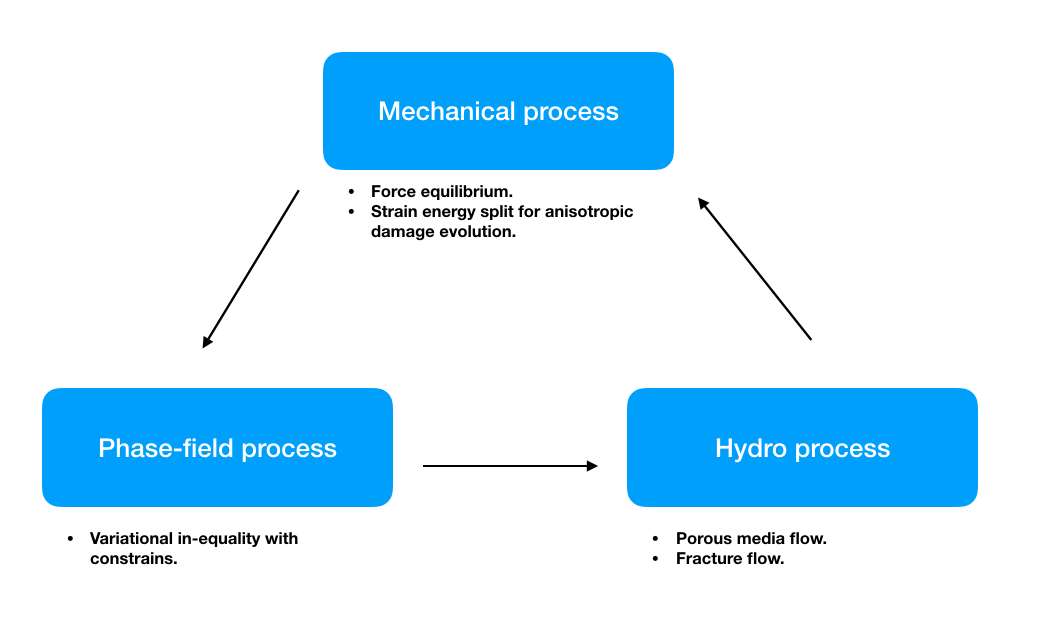
\includegraphics[width=0.9\textwidth]{figures/VPF_code.png}
\caption{Computation scheme with the variational phase-field model}
\label{fig:Keita_VPF_code}
\end{figure} 

The mechanical process solves the force equilibrium under the presence of the crack (damage) field in which the damage is accounted differently depending on the state of the load (e.g. compression or tension) in order to distinguish the material's response under different types of loading.
Various approaches have been proposed for the energy split strategy and the three of the most established approaches~\cite{Amor2009,Miehe2010a,Freddi2010} have been implemented.
Though the process for the phase-field is an elliptic problem, the solution space is bounded in $[0,1]$ and is constrained by the irreversibility (i.e. fracture is not allowed to heal).
Therefore, its solution requires a variational inequality solver and it is achieved through PETSc~\cite{petsc-user-ref, petsc-web-page}.
Once the displacement and the phase-field are solved, the crack opening displacement will be reconstructed following an approximation proposed by~\cite{Yoshioka2020} and the computation result will be passed onto the hydro process where fluid flows both in porous medium and fracture will be solved.
These processes will be repeated in a staggered manner until the convergence is met (currently its judgement is based on the phase-field process).
